\section{Anàlisis i preprocessat de dades}

\subsection{Preprocessat inicial}
Una vegada importem el dataset, es pot veure que hi ha bastantes cel·les buides i altres amb el string \texttt{`NaNN'}. Per solucionar aquesta inconsistència, s'han reemplaçat tots aquests valors per \texttt{pd.NA}. \\

Per altra banda, s'ha declarat el tipus de cada variable correctament (com a numèriques o com a categòriques) seguint la informació que es proporciona en el metadata file (que es pot trobar en \url{https://archive.ics.uci.edu/dataset/878/cirrhosis+patient+survival+prediction+dataset-1}).\\

Addicionalment, per una millor comprensió de les classes d'algunes variables, s'ha decidit reanomenar el seu \cite{misc_cirrhosis_patient_survival_prediction_878} 



Una vegada realitzats aquests canvis, es pot començar a treballar amb el dataset correctament.

\subsection{Anàlisis estadístic de les variables}
El primer que s'ha fet per entendre el dataset i poder treballar amb ell és realitzar un anàlisis estadístic de cada una de les variables que el formen. 

\subsubsection{Variables numèriques}
En les taules \ref{tab:num-stats-1} i \ref{tab:num-stats-2} es poden veure estadístiques sobre totes les variables numèriques del dataset (obtingudes mitjançant la comanda \texttt{data.describe()} de la llibreria \texttt{pandas}).

\begin{table}[H]
\centering
\begin{tabular}{|l|c|c|c|c|c|}
\hline
\textbf{} & \textbf{N\_Days} & \textbf{Age} & \textbf{Bilirubin} & \textbf{Cholesterol} & \textbf{Albumin} \\ \hline
\textbf{count} & 418.0 & 418.0 & 418.000000 & 284.0 & 418.000000 \\ \hline
\textbf{mean} & 1917.782297 & 18533.351675 & 3.220813 & 369.510563 & 3.497440 \\ \hline
\textbf{std} & 1104.672992 & 3815.845055 & 4.407506 & 231.944545 & 0.424972 \\ \hline
\textbf{min} & 41.0 & 9598.0 & 0.300000 & 120.0 & 1.960000 \\ \hline
\textbf{25\%} & 1092.75 & 15644.5 & 0.800000 & 249.5 & 
3.242500 \\ \hline
\textbf{50\%} & 1730.0 & 18628.0 & 1.400000 & 309.5 & 
3.530000 \\ \hline
\textbf{75\%} & 2613.5 & 21272.5 & 3.400000 & 400.0 & 
3.770000 \\ \hline
\textbf{max} & 4795.0 & 28650.0 & 28.000000 & 1775.0 & 
4.640000 \\ \hline
\end{tabular}
\caption{Estadístiques de les variables numèriques N\_Days, Age, Bilirubin, Cholesterol i Albumin.}
\label{tab:num-stats-1}
\end{table}

\begin{table}[H]
\centering
\begin{tabular}{|l|c|c|c|c|c|c|}
\hline
\textbf{} & \textbf{Copper} & \textbf{Alk\_Phos} & \textbf{SGOT} & \textbf{Triglycerides} & \textbf{Platelets} & \textbf{Prothrombin} \\ \hline
\textbf{count}     & 310.0           & 312.000000        & 312.000000    & 282.0                  & 407.0              & 416.000000           \\ \hline
\textbf{mean}      & 97.648387       & 1982.655769       & 122.55364     & 124.702128             & 257.02457          & 10.731731            \\ \hline
\textbf{std}       & 85.61392        & 2140.388824       & 56.699525     & 65.148639              & 98.325585          & 1.02200              \\ \hline
\textbf{min}       & 4.0             & 289.000000        & 26.350000     & 33.0                   & 62.0               & 9.00000              \\ \hline
\textbf{25\%}      & 41.25           & 871.500000        & 80.600000     & 84.25                  & 188.5              & 10.00000             \\ \hline
\textbf{50\%}      & 73.0            & 1259.000000       & 114.700000    & 108.0                  & 251.0              & 10.60000             \\ \hline
\textbf{75\%}      & 123.0           & 1980.000000       & 151.900000    & 151.0                  & 318.0              & 11.10000             \\ \hline
\textbf{max}       & 588.0           & 13862.400000      & 457.250000    & 598.0                  & 721.0              & 18.00000             \\ \hline
\end{tabular}
\caption{Estadístiques sobre les variables numèriques Copper, Alk\_Phos, SGOT, Triglycerides, Platelets i Prothrombin}
\label{tab:num-stats-2}
\end{table}

Addicionalment, en la figura \ref{fig:num-histograms-1} es poden veure les histogrames de cada una de les variables numèriques, on es veu la distribució de les seves dades ignorant els valors faltants (missings).

\begin{figure}
    \centering
    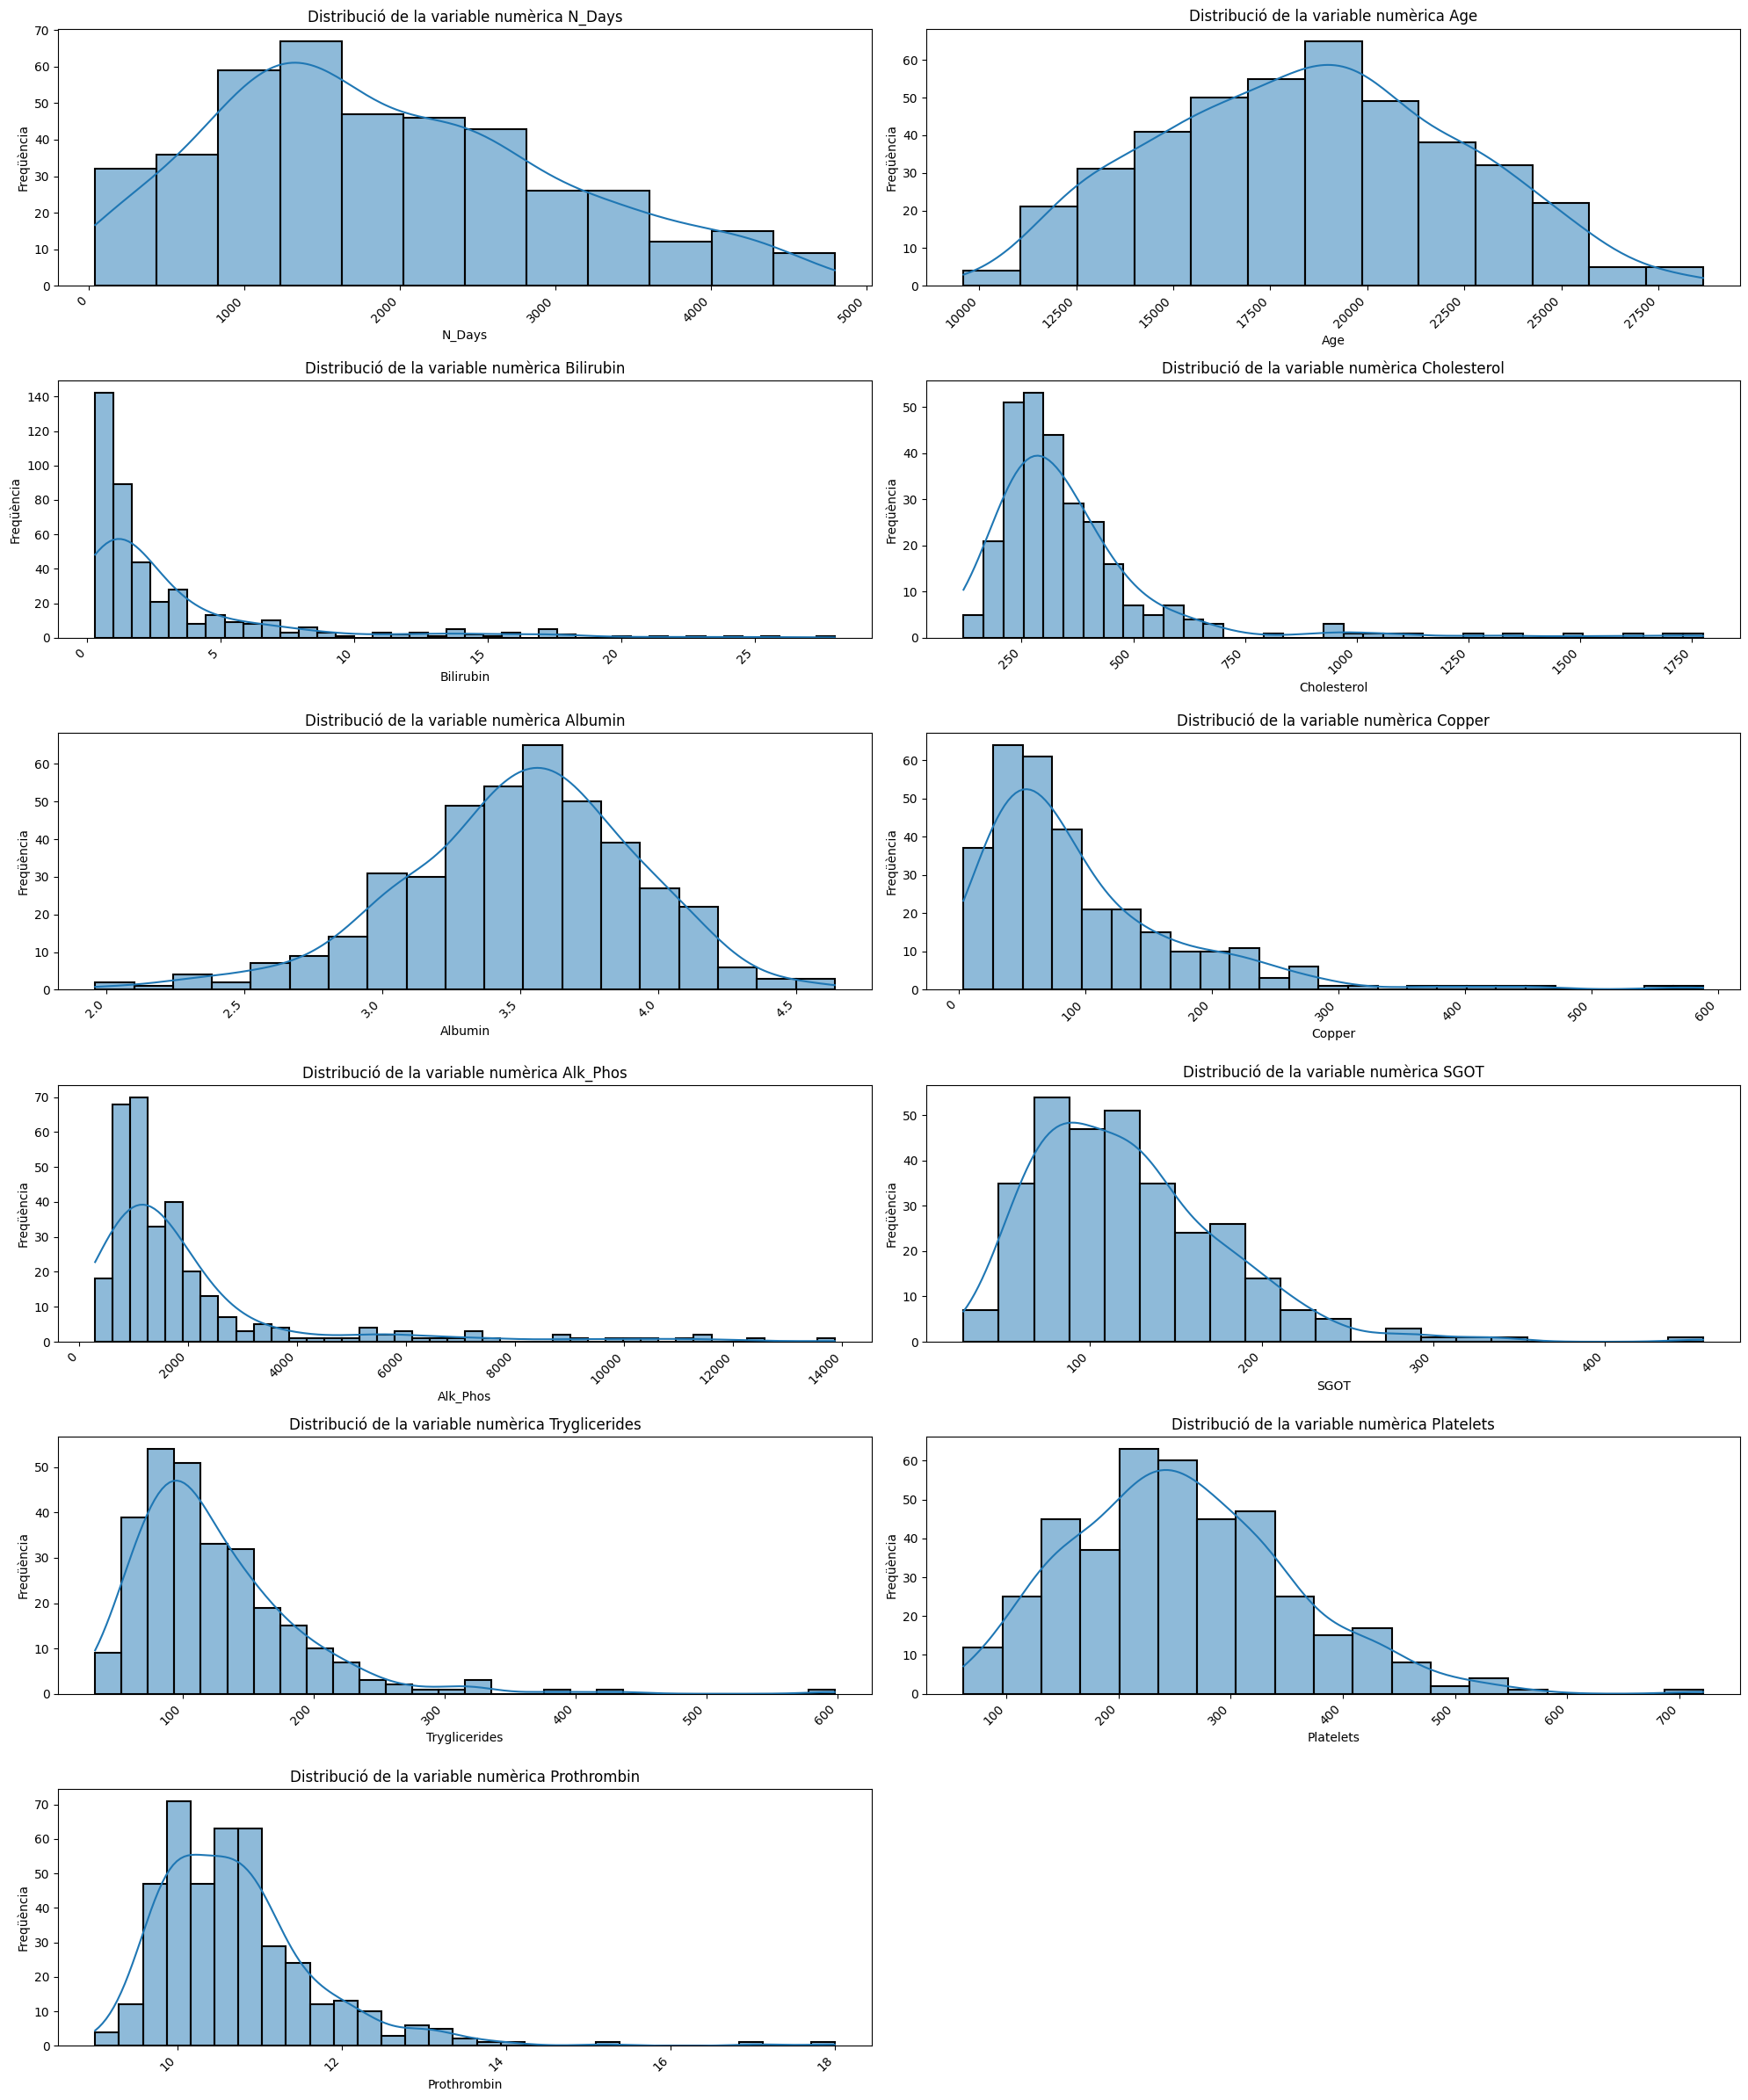
\includegraphics[width=\linewidth]{img/num-histograms.png}
    \caption{Histogrames de cada una de les variables numèriques del datset.}
    \label{fig:num-histograms-1}
\end{figure}

\subsubsection{Variables categòriques}
En les taules \ref{tab:cat-stats-1} i \ref{tab:cat-stats-2} podem veure altres estadístiques per les variables categòriques del dataset (obtingudes mitjançant la mateixa comanda, però amb el paràmetre \texttt{include=`category'}).

\begin{table}[H]
\centering
\begin{tabular}{|l|c|c|c|c|c|}
\hline
\textbf{} & \textbf{ID} & \textbf{Status} & \textbf{Drug} & \textbf{Sex} & \textbf{Ascites} \\ \hline
\textbf{count}     & 418         & 418             & 312            & 418           & 312              \\ \hline
\textbf{unique}    & 418         & 3               & 2              & 2             & 2                \\ \hline
\textbf{top}       & 1           & C               & D-penicillamine & F             & N                \\ \hline
\textbf{freq}      & 1           & 232             & 158            & 374           & 288              \\ \hline
\end{tabular}
\caption{Estadístiques sobre les variables categòriques ID, Status, Drug, Sex i Ascites.}
\label{tab:cat-stats-1}
\end{table}

\begin{table}[H]
\centering
\begin{tabular}{|l|c|c|c|c|}
\hline
\textbf{} & \textbf{Hepatomegaly} & \textbf{Spiders} & \textbf{Edema} & \textbf{Stage} \\ \hline
\textbf{count}     & 312                    & 312              & 418             & 412.0          \\ \hline
\textbf{unique}    & 2                      & 2                & 3               & 4.0            \\ \hline
\textbf{top}       & Y                      & N                & N               & 3.0            \\ \hline
\textbf{freq}      & 160                    & 222              & 354             & 155.0          \\ \hline
\end{tabular}
\caption{Estadístiques sobre les variabes categòriques Hepatomegaly, Spiders, Edema i Stage.}
\label{tab:cat-stats-2}
\end{table}

A més, en la figura \ref{fig:cat-countplots-1} es pot veure els countplots de cada una de les variables categòriques, on es veu la quantitat de mostres que hi ha per cada classe de la variable, evitant els valors faltants (missings).

\begin{figure}
    \centering
    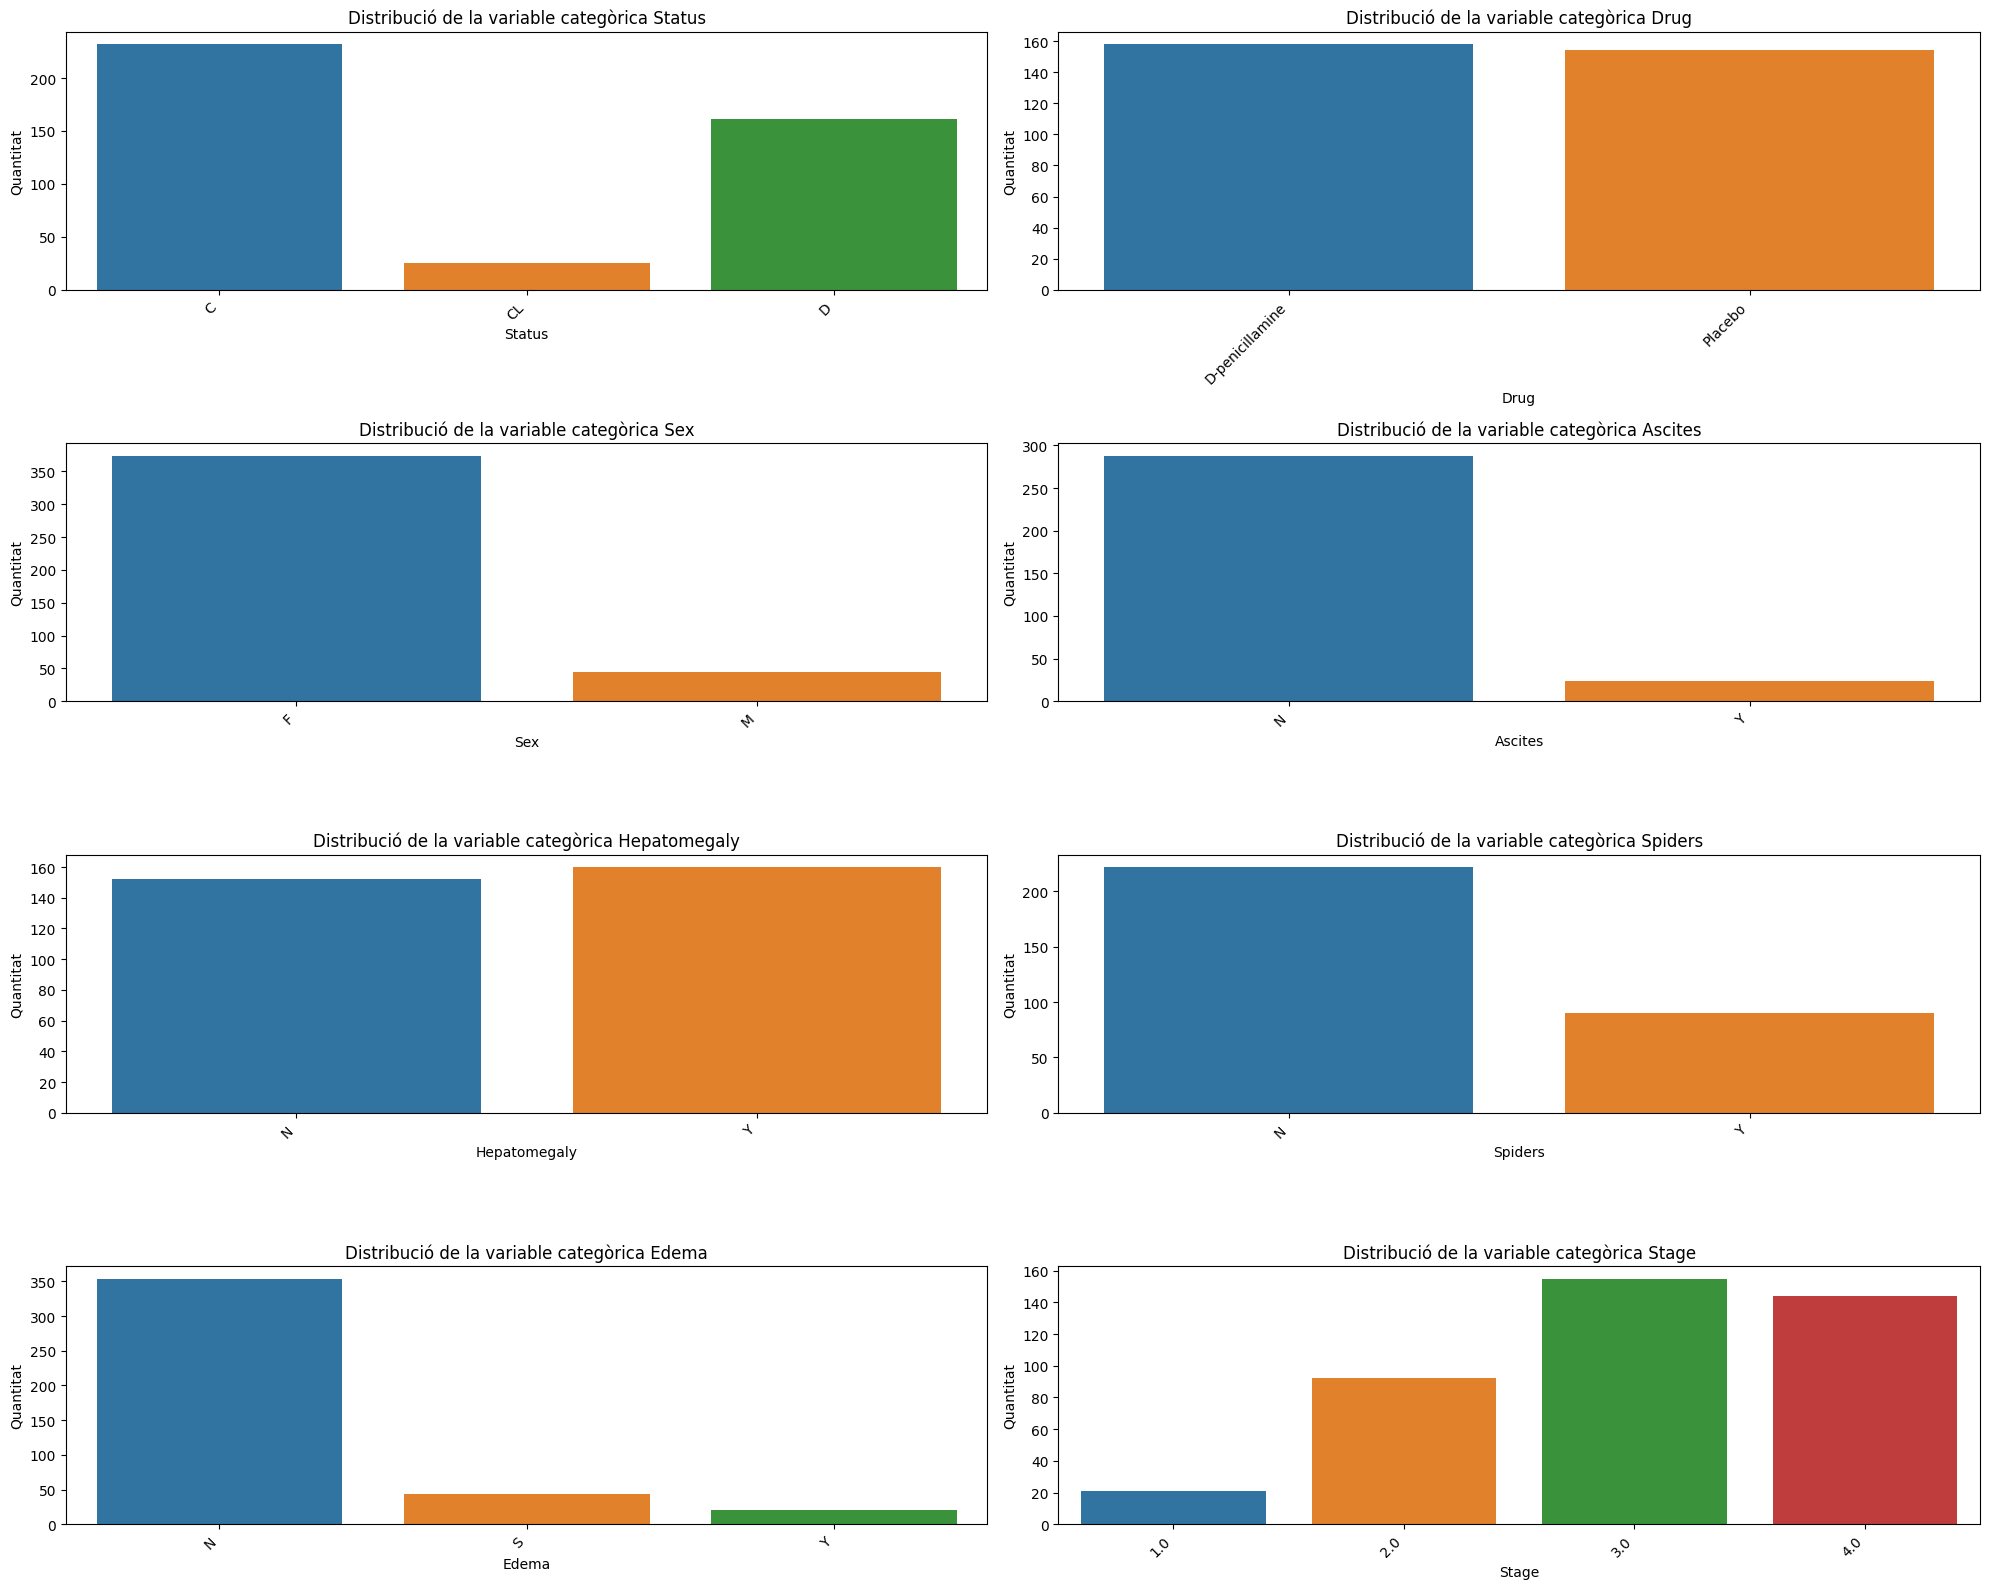
\includegraphics[width=\linewidth]{img/cat-countplots.png}
    \caption{Countplots de cada una de les variables categòriques del datset.}
    \label{fig:cat-countplots-1}
\end{figure}

\subsection{Estudi de balanceig de classes}

\subsection{Missings}

\subsection{Outliers}

\subsection{Recodificació de variables}

\subsection{Particionat del dataset}
%A partir d’aquest punt, no useu la partici ́o de validaci ́o (si heu decidit fer servir la partici ́o de validaci ́o) fins l’entrenament de models. La partici ́o de test no la podeu fer servir fins l’avaluaci ́o del model final. 1 Taula (mida de les particions). 
% –Si imputeu missings heu de particionar abans de la imputaci ́o.
%–Si feu servir un m`etode de balanceig heu de particionar abans de balancejar les classes